\documentclass[11pt,a4paper]{article}

\usepackage{style2017}
\usepackage{hyperref}

\hypersetup{
    colorlinks =false,
    linkcolor=blue,
   linkbordercolor = 1 0 0
}
\newcounter{numexo}
\setcellgapes{1pt}
\setlength{\parskip}{0.25cm}



\begin{document}



\begin{NSI}
{Activité}{Formulaire en HTML}
\end{NSI}

Les formulaires dans les pages web permettent de recueillir des informations et sont très utilisés. 

Dans le langage HTML, les balises \textsf{<form>}, \textsf{<input>} et \textsf{<label>} sont dédiées à la création des formulaires. 

\begin{center}
\includegraphics[scale=0.8]{img/formulaire_1.eps}
\end{center}

%Ces balises sont présentées dans la page de présentation qui se trouve dans le dossier à télécharger sur l'ENT.


\addtocounter{numexo}{1}
\subsection*{\Large Partie \thenumexo }

\begin{enumerate}
\item Sur le Moodle de l'ENT, récupérer l'archive formulaire.zip et la décompresser dans votre espace de travail.

\item Afficher la page web \textsf{presentation.html} et la lire pour connaître les principaux éléments d'un formulaire.

\item Ouvrir dans le même dossier la page \textsf{formulaire.html} et ajouter les éléments pour créer le formulaire ci-dessous:

\begin{center}
\includegraphics[scale=0.8]{img/formulaire_2.eps}
\end{center}

\item Afficher dans le navigateur le formulaire puis le compléter et valider.

\begin{enumerate}
\item Quelle est la méthode utilisée pour l'envoi du formulaire ? \vspace{2cm}

\item Est-il possible de connaître la méthode d'envoi du formulaire sans  éditer le code source ? Justifier.\vspace{2cm}

\item Où sont envoyées les données du formulaire ? \vspace{2cm}

\item Pourquoi le champ \textsf{nom} doit-il être complété ?\vspace{2cm}

\end{enumerate}

\item Modifier dans le code \textsf{html} la méthode d'envoi par \textbf{post} puis soumettre à nouveau le formulaire.
\begin{enumerate}
\item Quelle est la différence avec l'envoi précédent ?\vspace{2cm}

\item Les données sont-elles envoyées ? Justifier. \vspace{2cm}

\end{enumerate}

\item Ajouter au formulaire un champ de type \textsf{text} pour demander l'âge de l'utilisateur.
\begin{center}
\includegraphics[scale=0.8]{img/formulaire_3.eps}
\end{center}
\item Un formulaire peut contenir des boutons radios. L'ajout de ces boutons se fait avec des \textsf{input} de type \textsf{radio} et en ayant l'attribut \textsf{name} de même valeur. La page \textsf{présentation.html} contient un lien vers une documentation qui vous aidera.

L'attribut \textsf{name} doit être identique pour caque bouton radio et aura la valeur \textsf{pet}.
\begin{center}
\includegraphics[scale=0.8]{img/formulaire_4.eps}
\end{center}


\end{enumerate}

\newpage
\addtocounter{numexo}{1}
\subsection*{\Large Partie \thenumexo }

Les données du formulaire ne sont pas envoyées. Pour qu'un envoi soit possible, il faut un serveur qui héberge le formulaire et traite les données qui lui sont envoyées.

\begin{center}
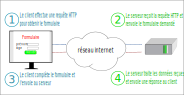
\includegraphics[scale=0.8]{img/client_serveur.eps}
\end{center}

On va installer un serveur WEB sur notre machine ou sur une clef USB avec l'application UwAmp disponible sur un partage réseau (voir avec le prof).

\begin{enumerate}
\item Installer le serveur UwAmp sur votre machine ou sur une clef USB.
\item Ouvrir le dossier \textsf{UwAmp} puis lancer l'application \textsf{UwAmp.exe}.

\begin{center}
\includegraphics[scale=0.7]{img/uwamp.eps}
\end{center}

\newpage
\item Ouvrir le dossier \textsf{www} avec le bouton \textbf{Dossier www} puis copier et coller tous les fichiers de formulaire et les dossiers (css, js, img) dans le dossier \textsf{my-app}.
\begin{center}
\includegraphics[scale=0.8]{img/dossier_my_app.eps}
\end{center}

\item Lancer le navigateur avec le bouton \textbf{Navigateur www}, rentrer dans le dossier \textsf{my-app} puis cliquer sur le fichier \textsf{formulaire.php}



\item On va étudier le comportement du formulaire.
\begin{enumerate}
\item Saisir un nom et un mot de passe au hasard. Que se passe-t-il ? \vspace{2cm}

\item Quelle est la méthode d'envoi utilisée par ce formulaire ?\vspace{2cm}


\item Saisir le nom \textsf{bob} et le mot de passe \textsf{eponge}. Quelle page est affichée ? \vspace{2cm}

\item Ouvrir la console de développement, activer l'onglet réseau et actualiser la page contenant le formulaire. Retrouver dans la console les données envoyées. Que remarquez-vous ?\vspace{2cm}

\item Que peut-on en déduire sur la sécurisation de la communication ?\vspace{2cm}
\end{enumerate}


\item On va éditer et modifier le formulaire. Attention, ce fichier mélange le langage \textsf{html} avec le langage de programmation \textsf{php}. Cette partie est donc difficile.

\begin{enumerate}

\item Le formulaire contient un attribut \textsf{action}. Quelle est la valeur de cet attribut pour notre formulaire ? \vspace{1cm}

\item Remplacer la méthode \textsf{post} par la méthode \textsf{get} et vérifier les modifications.

\item Modifier le fichier \textsf{formulaire.php} pour que le formulaire réponde favorablement à votre prénom et votre mot de passe.

\item Remplacer le champ \textsf{nom} par un champ \textsf{email} dans le fichier \textsf{formulaire.php}

\end{enumerate}


\end{enumerate}
\end{document}

